\section{Integration Strategy}
\subsection{Entry Criteria}
\subsection{Elements to be Integrated}
\subsection{Integration Testing Strategy}
The strategies we could use are: top-down, bottom-up, sandwich, thread and critical modules. After some considerations, we have understood that, among them, the preferable strategies are the first two ones written. Our choice depends on the three facts below:
	\begin{itemize}
		\item besides the sandwich strategy is flexible and adaptable, it's complicated to plan;
		\item it's not better to use the thread strategy: if we consider portions of several modules, some problems can occur because some modules depend on 		others, entirely and not only on a part of them.
		\item the critical modules strategy is more imprecised than the others.      
	\end{itemize} 
It's indifferent to use the bottom-up strategy or the top-down one. In this document, we have focused on the first strategy nominated.
\subsection{Sequence of Component/Function Integration}
\subsubsection{Integration Sequence}
Considering the bottom-up strategy, first of all, we will test the module called "Application Server", and, in particular, its submodules, represented in the image below:
    \begin{center}
	    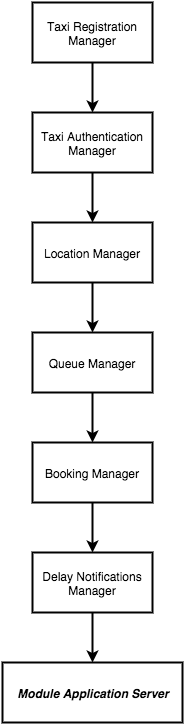
\includegraphics[width=0.28\textwidth]{./images/ModuleApplicationServer.png}~\\[1.5cm] 
    \end{center}	
After that, we can test two modules:
	\begin{itemize}
		\item the one named "Taxi Interface", represented in the image below
		    \begin{center}
			    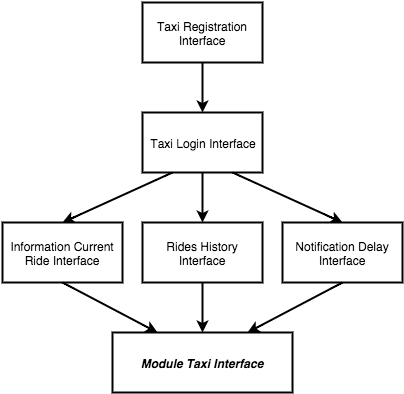
\includegraphics[width=0.60\textwidth]{./images/ModuleTaxiInterface.png}~\\[1.5cm] 
			\end{center}
		\item the one called "User Interface", corrisponding to the diagram below
		    \begin{center}
			    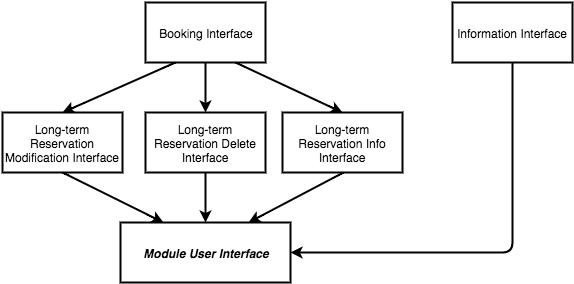
\includegraphics[width=0.85\textwidth]{./images/ModuleUserInterface.png}~\\[1.5cm] 
			\end{center}
	\end{itemize}
